% Header aus der Vorlage
\documentclass[a4paper,11pt, footheight=26pt]{scrartcl}
\usepackage[head=23pt]{geometry}	% head=23pt umgeht Fehlerwarnung, dafür größeres "top" in geometry
\geometry{a4paper, top=30mm, left=20mm, right=20mm, bottom=22mm,headsep=10mm, footskip=12mm}

% Input inkl. Umlaute, Silbentrennung
\usepackage[T1]{fontenc}
\usepackage[utf8]{inputenc}
\usepackage[ngerman]{babel}
\usepackage{csquotes}	% Anführungszeichen

% HTW Corporate Design: Arial (Helvetica)
\usepackage{helvet}
\renewcommand{\familydefault}{\sfdefault}

% Style-Aufhübschung
\usepackage{soul, color}	% Kapitälchen, Unterstrichen, Durchgestrichen usw. im Text
\usepackage{scrlayer-scrpage}	% Kopf-/Fußzeile
%\usepackage{titleref}
\usepackage[perpage]{footmisc}	% Fußnotenzählung Seitenweit, nicht Dokumentenweit

% Mathe usw.
\usepackage{amssymb}
\usepackage[fleqn]{amsmath}	% fleqn: align-Umgebung rechtsbündig
\usepackage{xcolor}
\usepackage{esint}	% Schönere Integrale, \oiint vorhanden
\everymath=\expandafter{\the\everymath\displaystyle}	% Mathe Inhalte werden weniger verkleinert
\usepackage{wasysym}	% mehr Symbole, bspw \lightning

% tikz usw.
\usepackage{tikz}
\usepackage{pgfplots}
\pgfplotsset{compat=1.11}	% Umgeht Fehlermeldung
\usetikzlibrary{graphs}
%\usetikzlibrary{through}	% ???
\usetikzlibrary{arrows}
\usetikzlibrary{arrows.meta}	% Pfeile verändern / vergrößern: \draw[-{>[scale=1.5]}] (-3,5) -> (-3,3);
\usetikzlibrary{automata,positioning} % Zeilenumbruch im Node node[align=center] {Text\\nächste Zeile}
\usetikzlibrary{patterns}	% Schraffierte Füllung
\tikzstyle{reverseclip}=[insert path={	% Inverser Clip \clip
	(current page.north east) --
	(current page.south east) --
	(current page.south west) --
	(current page.north west) --
	(current page.north east)}
% Nutzen: 
%\begin{tikzpicture}[remember picture]
%\begin{scope}
%\begin{pgfinterruptboundingbox}
%\draw [clip] DIE FLÄCHE, IN DER OBJEKT NICHT ERSCHEINEN SOLL [reverseclip];
%\end{pgfinterruptboundingbox}
%\draw DAS OBJEKT;
%\end{scope}
%\end{tikzpicture}
]	% Achtung: dafür muss doppelt kompliert werden!
\usepackage{graphpap}	% Grid für Graphen

% Tabular
\usepackage{longtable}	% Große Tabellen über mehrere Seiten
\usepackage{multirow}	% Multirow/-column: \multirow{2[Anzahl der Zeilen]}{*[Format]}{Test[Inhalt]} oder \multicolumn{7[Anzahl der Reihen]}{|c|[Format]}{Test2[Inhalt]}
\renewcommand{\arraystretch}{1.3} % Tabellenlinien nicht zu dicht
\usepackage{colortbl}
\arrayrulecolor{gray}	% heller Tabellenlinien

% Nützliches
\usepackage{verbatim}	% u.a. zum auskommentieren via \begin{comment} \end{comment}
\usepackage{tabto}	% Tabs: /tab zum nächsten Tab oder /tabto{.5 \CurrentLineWidth} zur Stelle in der Linie
\NumTabs{6}	% Anzahl von Tabs pro Zeile zum springen
\usepackage{listings} % Source-Code mit Tabs
\usepackage{lstautogobble} 
\usepackage{enumitem}	% Anpassung der enumerates
\setlist[enumerate,1]{label=\arabic*.)}	% global andere Enum-Items
\usepackage{letltxmacro} % neue Definiton von Grundbefehlen
% Nutzen:
%\LetLtxMacro{\oldemph}{\emph}
%\renewcommand{\emph}[1]{\oldemph{#1}}

% Einrichtung von lst
\lstset{
basicstyle=\ttfamily, 
mathescape=true, 
escapeinside=||, 
autogobble, 
tabsize=2,
basicstyle=\footnotesize\sffamily\color{black},
frame=single,
rulecolor=\color{lightgray},
numbers=left,
numbersep=5pt,
%basicstyle=\footnotesize\sffamily\color{black},
commentstyle=\color{gray},
%frame=single,
%numbers=left,
%numbersep=5pt,
numberstyle=\tiny\color{gray},
keywordstyle=\color{green},
%showspaces=false,
showstringspaces=false,
stringstyle=\color{orange},
tabsize=2,
literate=%
    {Ö}{{\"O}}1
    {Ä}{{\"A}}1
    {Ü}{{\"U}}1
    {ß}{{\ss}}1
    {ü}{{\"u}}1
    {ä}{{\"a}}1
    {ö}{{\"o}}1
    {~}{{\textasciitilde}}1
}

% BibTeX
\usepackage[backend=bibtex, bibencoding=ascii]{biblatex}	% BibTeX
\usepackage{makeidx}
%\makeglossary
%\makeindex

% Grafiken
\usepackage{graphicx}
\usepackage{epstopdf}	% eps-Vektorgrafiken einfügen

% pdf-Setup
\usepackage{pdfpages}
\usepackage[bookmarks,%
bookmarksopen=false,% Klappt die Bookmarks in Acrobat aus
colorlinks=true,%
linkcolor=black,%
citecolor=red,%
urlcolor=green,%
]{hyperref}

% Titel, Autor usw. werden vor dem Anfang des Dokuments in einem Rutsch definiert…
\newcommand{\DTitel}[1]{\newcommand{\Dokumententitel}{#1}}
\newcommand{\DUntertitel}[1]{\newcommand{\Dokumentenuntertitel}{#1}}
\newcommand{\DAutor}[1]{\newcommand{\Dokumentenautor}{#1}}
\newcommand{\DNotiz}[1]{\newcommand{\Dokumentennotiz}{#1}}
% … Deswegen folgendes erst Nach Dokumentenbeginn ausführen:
\AtBeginDocument{
	\hypersetup{
		pdfauthor={\Dokumentenautor},
		pdftitle={HTW Dresden | \Dokumententitel - \Dokumentenuntertitel},
	}
	\automark[section]{section}
	\automark*[subsection]{subsection}
	\pagestyle{scrheadings}
	\ihead{
\includegraphics[height=1.7em]{../LaTeX_master/HTW-Logo.eps}}
	\ohead{\Dokumententitel}
	\ofoot{\footnotesize{\textcolor{darkgray}{Mitschrift von\\ \Dokumentenautor}}}
	% Titelseite
	\title{
\includegraphics[width=0.35\textwidth]{../LaTeX_master/HTW-Logo.eps}\\\vspace{0.5em}
	\Huge\textbf{\Dokumententitel} \\\vspace*{0,5cm}
	\Large \Dokumentenuntertitel \\\vspace*{4cm}}
	\author{\textcolor{darkgray}{Mitschrift von \Dokumentenautor} \vspace*{1cm}\\\Dokumentennotiz}
}

%% EIGENE BEFEHLE

%Farbdefinitionen
\definecolor{red}{RGB}{180,0,0}
\definecolor{green}{RGB}{75,160,0}
\definecolor{blue}{RGB}{0,75,200}
\definecolor{orange}{RGB}{255,128,0}
\definecolor{yellow}{RGB}{255,245,0}
\definecolor{purple}{RGB}{75,0,160}
\definecolor{cyan}{RGB}{0,160,160}
\definecolor{brown}{RGB}{120,60,10}

% Textfarbe ändern
\newcommand{\tred}[1]{\textcolor{red}{#1}}
\newcommand{\tgreen}[1]{\textcolor{green}{#1}}
\newcommand{\tblue}[1]{\textcolor{blue}{#1}}
\newcommand{\torange}[1]{\textcolor{orange}{#1}}
\newcommand{\tyellow}[1]{\textcolor{yellow}{#1}}
\newcommand{\tpurple}[1]{\textcolor{purple}{#1}}
\newcommand{\tcyan}[1]{\textcolor{cyan}{#1}}
\newcommand{\tbrown}[1]{\textcolor{brown}{#1}}

% Umstellen der Tabellen Definition
\newcommand{\mpb}[1][.3]{\begin{minipage}{#1\textwidth}\vspace*{3pt}}
\newcommand{\mpe}{\vspace*{3pt}\end{minipage}}

\newcommand{\resultul}[1]{\underline{\underline{#1}}}
\newcommand{\parskp}{$ $\\}	% new line after paragraph
\newcommand{\corr}{\;\widehat{=}\;}
\newcommand{\mdeg}{^{\circ}}

\newcommand{\nok}[2]{\begin{pmatrix}#1\\#2\end{pmatrix}}	% n über k

%\bibliography{../Literatur/HTW_Literatur.bib}

% Definition von Titel, Autor usw.
\DTitel{Datenbanksysteme I}
\DUntertitel{Vorlesungsskript}
\DAutor{Falk-Jonatan Strube}
\DNotiz{Vorlesung von Dr. Axel Toll}

\begin{document}

\maketitle
\newpage
\tableofcontents
\newpage

\section*{Prüfungsmodalitäten}
\paragraph{PVL} unbenoteter Beleg als Voraussetzung zur Prüfung
\begin{enumerate}
\item Access-Beleg (in Papier-Form abzugeben)
\item Abnahme der SQL-Praktikums-Aufgaben (Abnahme während Praktikumszeit)
\end{enumerate}

\paragraph{SP} schriftliche Prüfung, 90min\\
keine eigenen Unterlagen zugelassen. Nur zuvor ausgegeben Referenzen.

\section[Datenbank als System und Modell]{Betriebliche Informations- und Kommunikationssysteme - Unternehmensmodell - Datenbank}

\subsection{Daten als Unternehmensressource}
\subsubsection{Daten und Informationen}
Redundante Daten bergen Gefahr von Inkonsistenz $\Rightarrow$ Ziel: Schaffen von Datenbank mit folgenden Eigenschaften:
\begin{itemize}
\item ohne Inkonsistenzen (redundanzarm)
\item Zugriffsschutz
\item Mehrfachzugriff
\item Backup-Möglichkeiten (mit Widerspruchsfreier Wiederherstellung)
\end{itemize}

\begin{center}
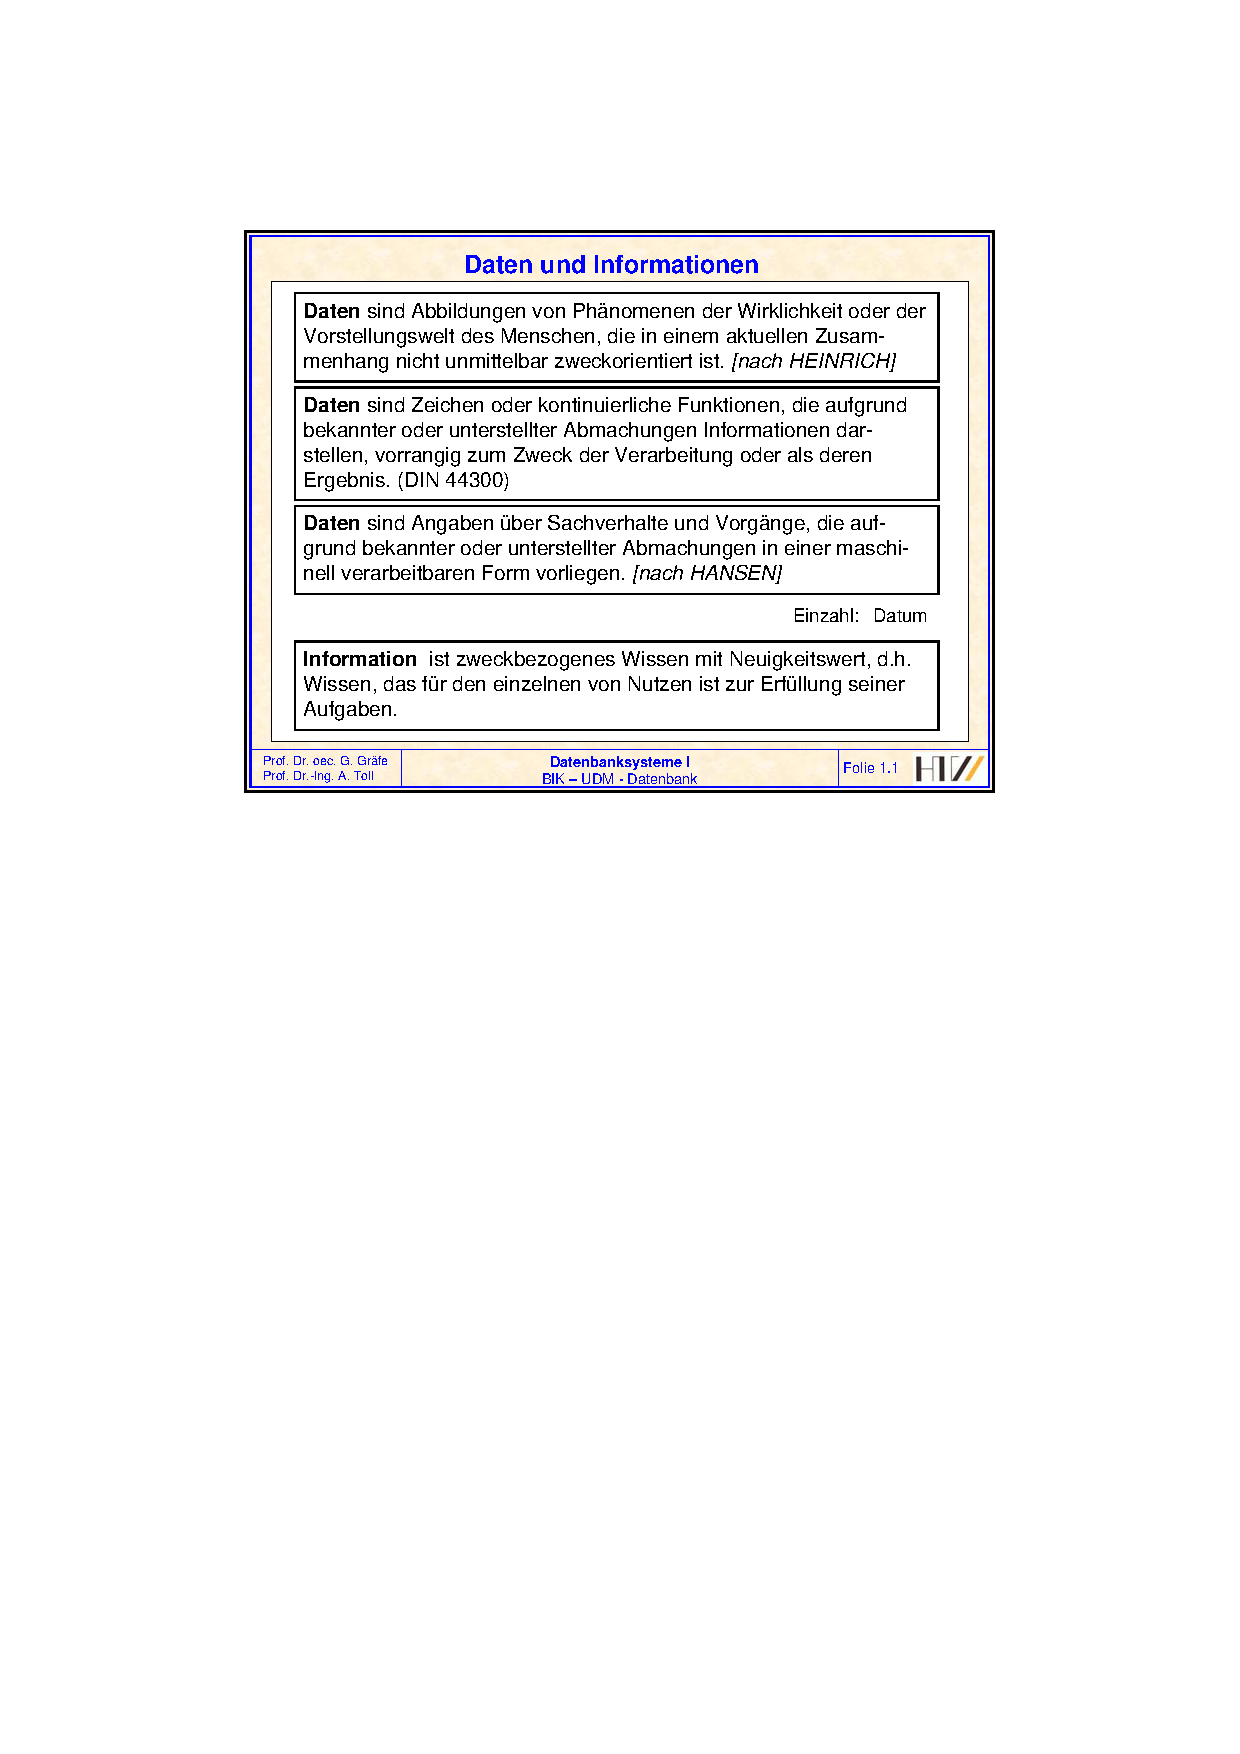
\includegraphics[page=1]{Vorlesung/oneperpage/Kap1_BIK_UDM_Datenbank.pdf}
\end{center}
%\subparagraph{Folie 1.1}\parskp
\begin{tabular}{r | c c}
& Daten & Informationen\\
\hline
Zweck & zweckneutral & zweckgebunden\\
Verarbeitung & maschinell & Interpretation durch Menschen\\
Speicherform & vergegenständlicht & an Menschen gebunden\\
\end{tabular}
\paragraph{Betriebliche Produktionsfaktoren}
\begin{itemize}
\item klassische Faktoren
\begin{itemize}
\item Betriebsmittel
\item Werkstoffe
\item Arbeitskraft
\end{itemize}
\item Daten + Informationen
\end{itemize}

\begin{center}
\includegraphics[page=2]{Vorlesung/oneperpage/Kap1_BIK_UDM_Datenbank.pdf}
\end{center}
%\subparagraph{Folie 1.2}\parskp
Große Datenbestände $\Rightarrow$ Maßnahmen zur Datenorganisation\bigskip\\
Eine mögliche Organisationsform (logisches Konzept): Ablage in Relationen (=Tabelle)\bigskip\\
Eine Zeile in dieser Tabelle nennt man \emph{Datensatz} (Tupel, Record, …).\\
Eine Spalte nennt man Datenfeld.

\subsubsection{Klassifikation von Daten}
\paragraph{Mögliche Kriterien} für Datenfeld
\begin{itemize}
\item Zeichenart
\begin{itemize}
\item ganze Zahl $\Rightarrow$ für Aufzählungen
\item reelle zahl $\Rightarrow$ numerische Berechnungen
\item Währung $\Rightarrow$ finanztechnische Berechnungen
\item Datum $\Rightarrow$ kalendarische Berechnungen/Werte
\item Text $\Rightarrow$ Beschreibung
\item Bitmuster $\Rightarrow$ Video, Bilder, …
\end{itemize}
\item Erscheinungsform
\begin{itemize}
\item sprachlich
\item bildlich
\item schriftlich
\end{itemize}
\item Stellung im Verarbeitungsprozess (E - V - A)
\begin{itemize}
\item Eingabe
\item Verarbeitung
\item Ausgabe
\end{itemize}
\item Verarbeitbarkeit mittels IT\\
(Umwandlung in digitale Daten: analog $\rightarrow$ diskret $\rightarrow$ digital)
\item Verwendungszweck\\
\begin{tabular}{
p{\dimexpr0.2\columnwidth-2\tabcolsep-1.5\arrayrulewidth} | >{\raggedright}
p{\dimexpr0.4\columnwidth-2\tabcolsep-1.5\arrayrulewidth} | >{\raggedright}
p{\dimexpr0.3\columnwidth-2\tabcolsep-1.5\arrayrulewidth}}
& Charakterisierung & Beispiel\tabularnewline
\hline
Stammdaten & selten zu verändern (über längeren Zeitraum in Struktur und Inhalt konstant) & Personalstammdaten (Name, Adresse)\tabularnewline
Änderungsdaten & Aktualisierung der Stammdaten & Änderung der Adresse\tabularnewline
Bestandsdaten & Periodische Änderung des wertes (Inhalt) von Feldern, Datenstruktur besteht über längeren Zeitraum konstant & Lagerbestände, Kassenbestände\tabularnewline
Bewegungsdaten & Daten zur Aktualisierung des Wertes von Bestandsdaten & Lagerzugänge und -abgänge\tabularnewline
Archivdaten & vergangenheitsbezogene Daten die über langeren Zeitraum aufbewahrt werden & Rechnungen, Buchungen der vergangenen 5 Jahre\tabularnewline
Transferdaten & Daten, die von einem anderen Programm erzeugt wurden und an ein anderes transferiert werden & Verkauf von Kundenadresson\tabularnewline
Vormerkdaten & Daten, die solange existieren, bis ein genau definiertes Ereignis eintritt & Reservierung einer Materialmenge im Lager
\end{tabular}
\end{itemize}

\subsubsection{Datenverschlüsselung}
Gemeint ist nicht die Codierung und Decodierung von Daten, sondern das Zuweisen von Schlüsseln zu Datensätzen.
\begin{center}
\includegraphics[page=3]{Vorlesung/oneperpage/Kap1_BIK_UDM_Datenbank.pdf}
\end{center}
%\paragraph{Folie 1.3}
\paragraph{Identifizierender Schlüssel} \parskp
kennzeichnet Objekteindeutig\\
Bsp.:
\begin{itemize}
\item Personal-Nr.
\item Material-Nr.
\end{itemize}
\paragraph{Klassifiziernder Schlüssel} \parskp
ordnet Objekt einer Klasse zu\\
Bsp.:
\begin{itemize}
\item Länderkennung: D, C, CH, …
\item Geschlecht: M, W
\end{itemize}
\paragraph{Hierarchischer Verbundschlüssel} \parskp
identifizierender Teil hängt vom klassifizierenden Teil ab\\
Bsp.:
\begin{itemize}
\item Autokennzeichen: $\underbrace{\text{DD}}_{\text{klass.}} \underbrace{\text{XY 715}}_{\text{ident.}}$
\end{itemize}
\paragraph{Parallelschlüssel} \parskp
zwei unabhängige Schlüsselteile\\
Bsp.:
\begin{itemize}
\item Flugnummer $\underbrace{\text{LH 283}}_{\text{Flugnr.}} \underbrace{\text{AB3}}_{\text{Flugzeug}}$
\end{itemize}
\begin{center}
\includegraphics[page=4]{Vorlesung/oneperpage/Kap1_BIK_UDM_Datenbank.pdf}
\end{center}
%\paragraph{Folie 1.4}




%\newpage
%\printbibliography
\end{document}